\chapter{Architectural design} \label{chap:architectural}


\section{Overview}
This chapter, arguably the longest of this document, analyses different aspects of the architecture of myTaxiService system. In \cref{sec:highlevel} we give a high level description of the structure of the system; inevitably this section will be pretty theoretical.

Then in \cref{sec:componentView} we focus on the components of the system. With the word \emph{component} we refer to an independent software element that encapsulates a set of related functions, namely that is defined by its interfaces. The interfaces between the components are fully analysed in \cref{sec:componentInterfaces}. In opposition to the focus on the interactions within the system, the deployment view in \cref{sec:deployment} provides further details on the structure of its various parts.

In the runtime view (\cref{sec:runtime}) we show the behaviour of the system in case of a request and a reservation. 

Finally, \cref{sec:styles} and \cref{sec:decisions} are meant to give further details and explanations about our design and architectural choices.

In the whole chapter, we will make extensive use of UML diagrams, UML being an agreed and relatively easy to understand language.


\section{High level components and their interaction}\label{sec:highlevel}
%[JavaEE architecture > see Quinton]

%[here you can introduce the high level components of your architecture (in our basic example in the slides about design you find these in slide 7) and describe the main interaction between them (no details here. You can say why some components talk to each other, why, if the communication is synchronous or asynchronous, any other info you think is useful at this point).]

For our myTaxiService ecosystem, we will adopt the Java Enterprise Edition (Java EE) application model for enterprise applications. This will allow the design, building and production of a solid, fast and reliable system, with a special focus on money and resources. 

\begin{figure}%
	\centering%
	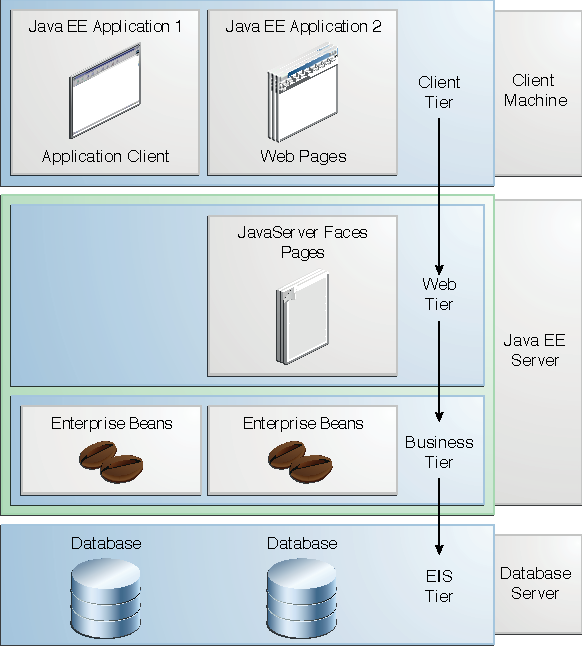
\includegraphics[width=0.85\linewidth]{img/JEETT}%
	\caption{High level architecture. Source: \emph{Java Platform, Enterprise Edition. The Java EE Tutorial, Release 7}. Oracle, September 2014.}\label{fig:jeett}%
\end{figure}

The Java EE platform uses a distributed multitiered application model, shown in \cref{fig:jeett}. Application logic is divided into components according to function (these will be detailed further in the chapter), and the application components that make up a Java EE application are installed on various machines depending on the tier to which the application component belongs. \Cref{fig:jeett} shows the model we will adopt, which consists of four tiers:

\begin{description}
	\item [Client tier] it contains all the components which run on the client machine (applications, web pages); in our case myTaxiWeb web pages, and myTaxiApp, myTaxiAssist mobile applications are the clients. These are all \emph{thin clients}, which means that they do not directly query the database, nor execute complex operations. 
	
	\item [Web tier] the components of this tier run on the Java EE server; this tier is intended to mange the data flow between clients and Java EE server and between server components and the database.

	\item [Business tier] this tier, which runs on the Java EE server as well, contains the so called \emph{enterprise beans}. Enterprise beans handle business code, which is logic that govern myTaxiService system; to do so, they also retrieve data from storage, processes it (if necessary), and sends it back to the client program.

	\item [EIS tier] this tier, typically, handles EIS\footnote{EIS stands for Enterprise information system.} software and includes enterprise infrastructure systems, such as enterprise resource planning (ERP), mainframe transaction processing, database systems, and other legacy information systems. In our specific case, Java EE application components might need access to enterprise information systems for database connectivity.
	
\end{description}













\section{Component view}\label{sec:componentView}
%[here you have a refinement of what you have in Section 4.B and identify sub-components. For instance, the diagram in slide 6 could be a diagram showing a  component view]

Now let us refine what was given in \cref{sec:highlevel}. In the following component diagram (\cref{fig:component}) the architecture of the system has been expanded.

\begin{figure*}%
	\centering%
	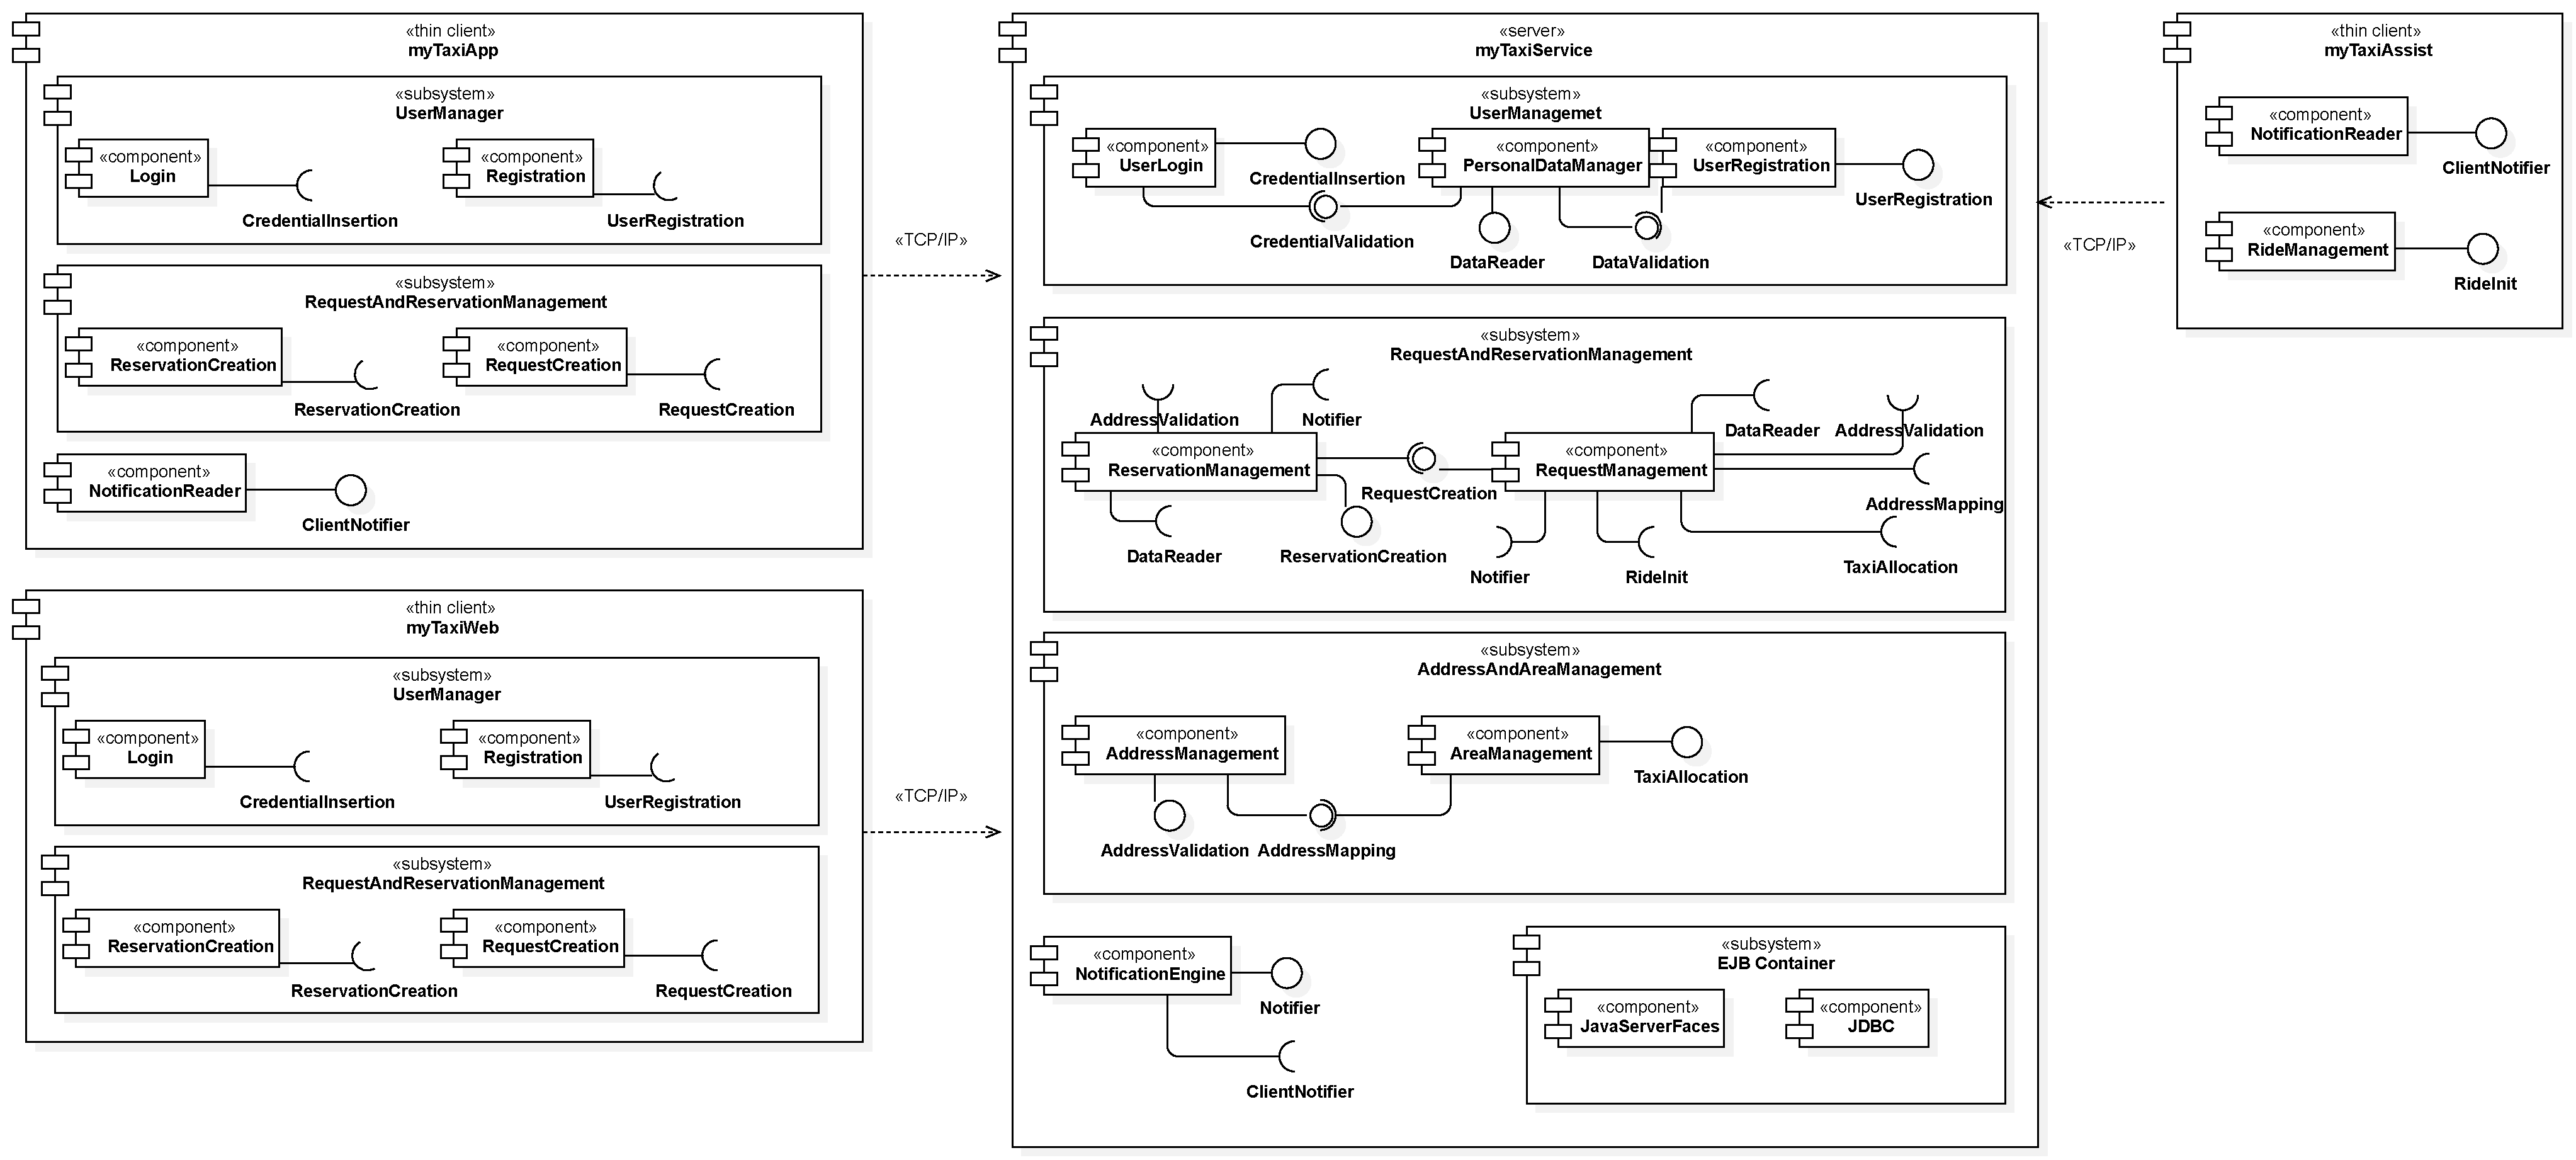
\includegraphics[width=\linewidth]{img/ComponentView__ComponentDiagram_1}%
	\caption{Component diagram.}\label{fig:component}%
\end{figure*}

In the diagram, each application of the system (myTaxiApp, myTaxiWeb, myTaxiAssist, myTaxiService) is represented, together with its own components. Moreover, for the sake of clarity, some subsystems have been introduced, to gather logically similar components. Each component may offer or require some interfaces. These interfaces reflect the services that the component provides (which are indicated in UML by a circle at the end of a line from the component icon) and the services that the component requires to operate correctly (the symbol for this kind of interface is a semicircle at the end of a line from the component icon).

For example, let us consider the \texttt{Re\-quest\-And\-Res\-er\-va\-tion\-Man\-age\-ment} subsystem in myTaxiService server. It has two components, \texttt{Res\-er\-va\-tion\-Man\-age\-ment} and \texttt{Re\-quest\-Man\-age\-ment}. The former, as the name suggests, handles the reservations, from the reception until their conversion to requests (remember that our system confirms the reservation and allocates a taxi \num{10} minutes before the meeting time with the customer, as though it was a request). In order to do the conversion, the component needs a service, namely \texttt{Re\-quest\-Cre\-ation}, which is offered by \texttt{Re\-quest\-Man\-age\-ment} component.

For the sake of clarity, we preferred to draw only the connections between the applications, and to exclude all the links between interfaces that would lie outside the subsystems. By doing so, we avoid the otherwise inevitable tangle of connections. Further details about the interfaces are provided in \cref{sec:componentInterfaces}.

Before we proceed with our analysis, we would like to focus our attention on \texttt{EJB Con\-tain\-er} subsystem. It provides all the JavaBeans components\footnote{\emph{JavaBeans} denotes a set of standards and conventions useful to build components in Java language.} which are essential for the operation of the system. Among them, we rely in particular on \texttt{Java\-Ser\-ver\-Faces}, to handle the server side for the clients, and on \texttt{Java\-Per\-sist\-ence\-API}, which makes the usage of MySQL database management system possible.


%%%%%%%%%%%%%%%%%%%%%%%%%%%%%%%%%%%%%%%%%%%%%%%%%%%%%%%%%%%%%%%%%%%%%%%%
%TODO Particolare nota al subsystem EJB Container, che contiene quei JavaBeans ritenuti indispensabili per il corretto funzionamento del sistema, tra i quali Java Server Faces, lato server del web client, e tutte le funzionalità offerte da Java Persistence API (nel diagramma è indicato come JDBC, provvederò a correggere, ricordamelo!), per l’utilizzo del DB MySQL. ANCHE IN RUNTIME, DEPLOYMENT?
%%%%%%%%%%%%%%%%%%%%%%%%%%%%%%%%%%%%%%%%%%%%%%%%%%%%%%%%%%%%%%%%%%%%%%%%


\section{Component interfaces}\label{sec:componentInterfaces}
\textbf{[communication between components] [here you define the interfaces of your components, that is, which operations they offer to the external world, their meaning, any input and output parameter (name, possible set of values/type)]}

\lipsum[1-5]













\clearpage%TODO Remove.
\section{Deployment view}\label{sec:deployment}
%[this is what you have in slide 8, that is, the identification of the artifact that need to be deployed to have the system working]

After focusing on the logical structure of the system, in the component view, and on the interactions within the system, it is appropriate to provide a lower level view on the architecture of the system. In particular the deployment diagram in \cref{fig:deployment} shows the distribution of the components over the various hardware devices.

\begin{figure*}%
	\centering%
	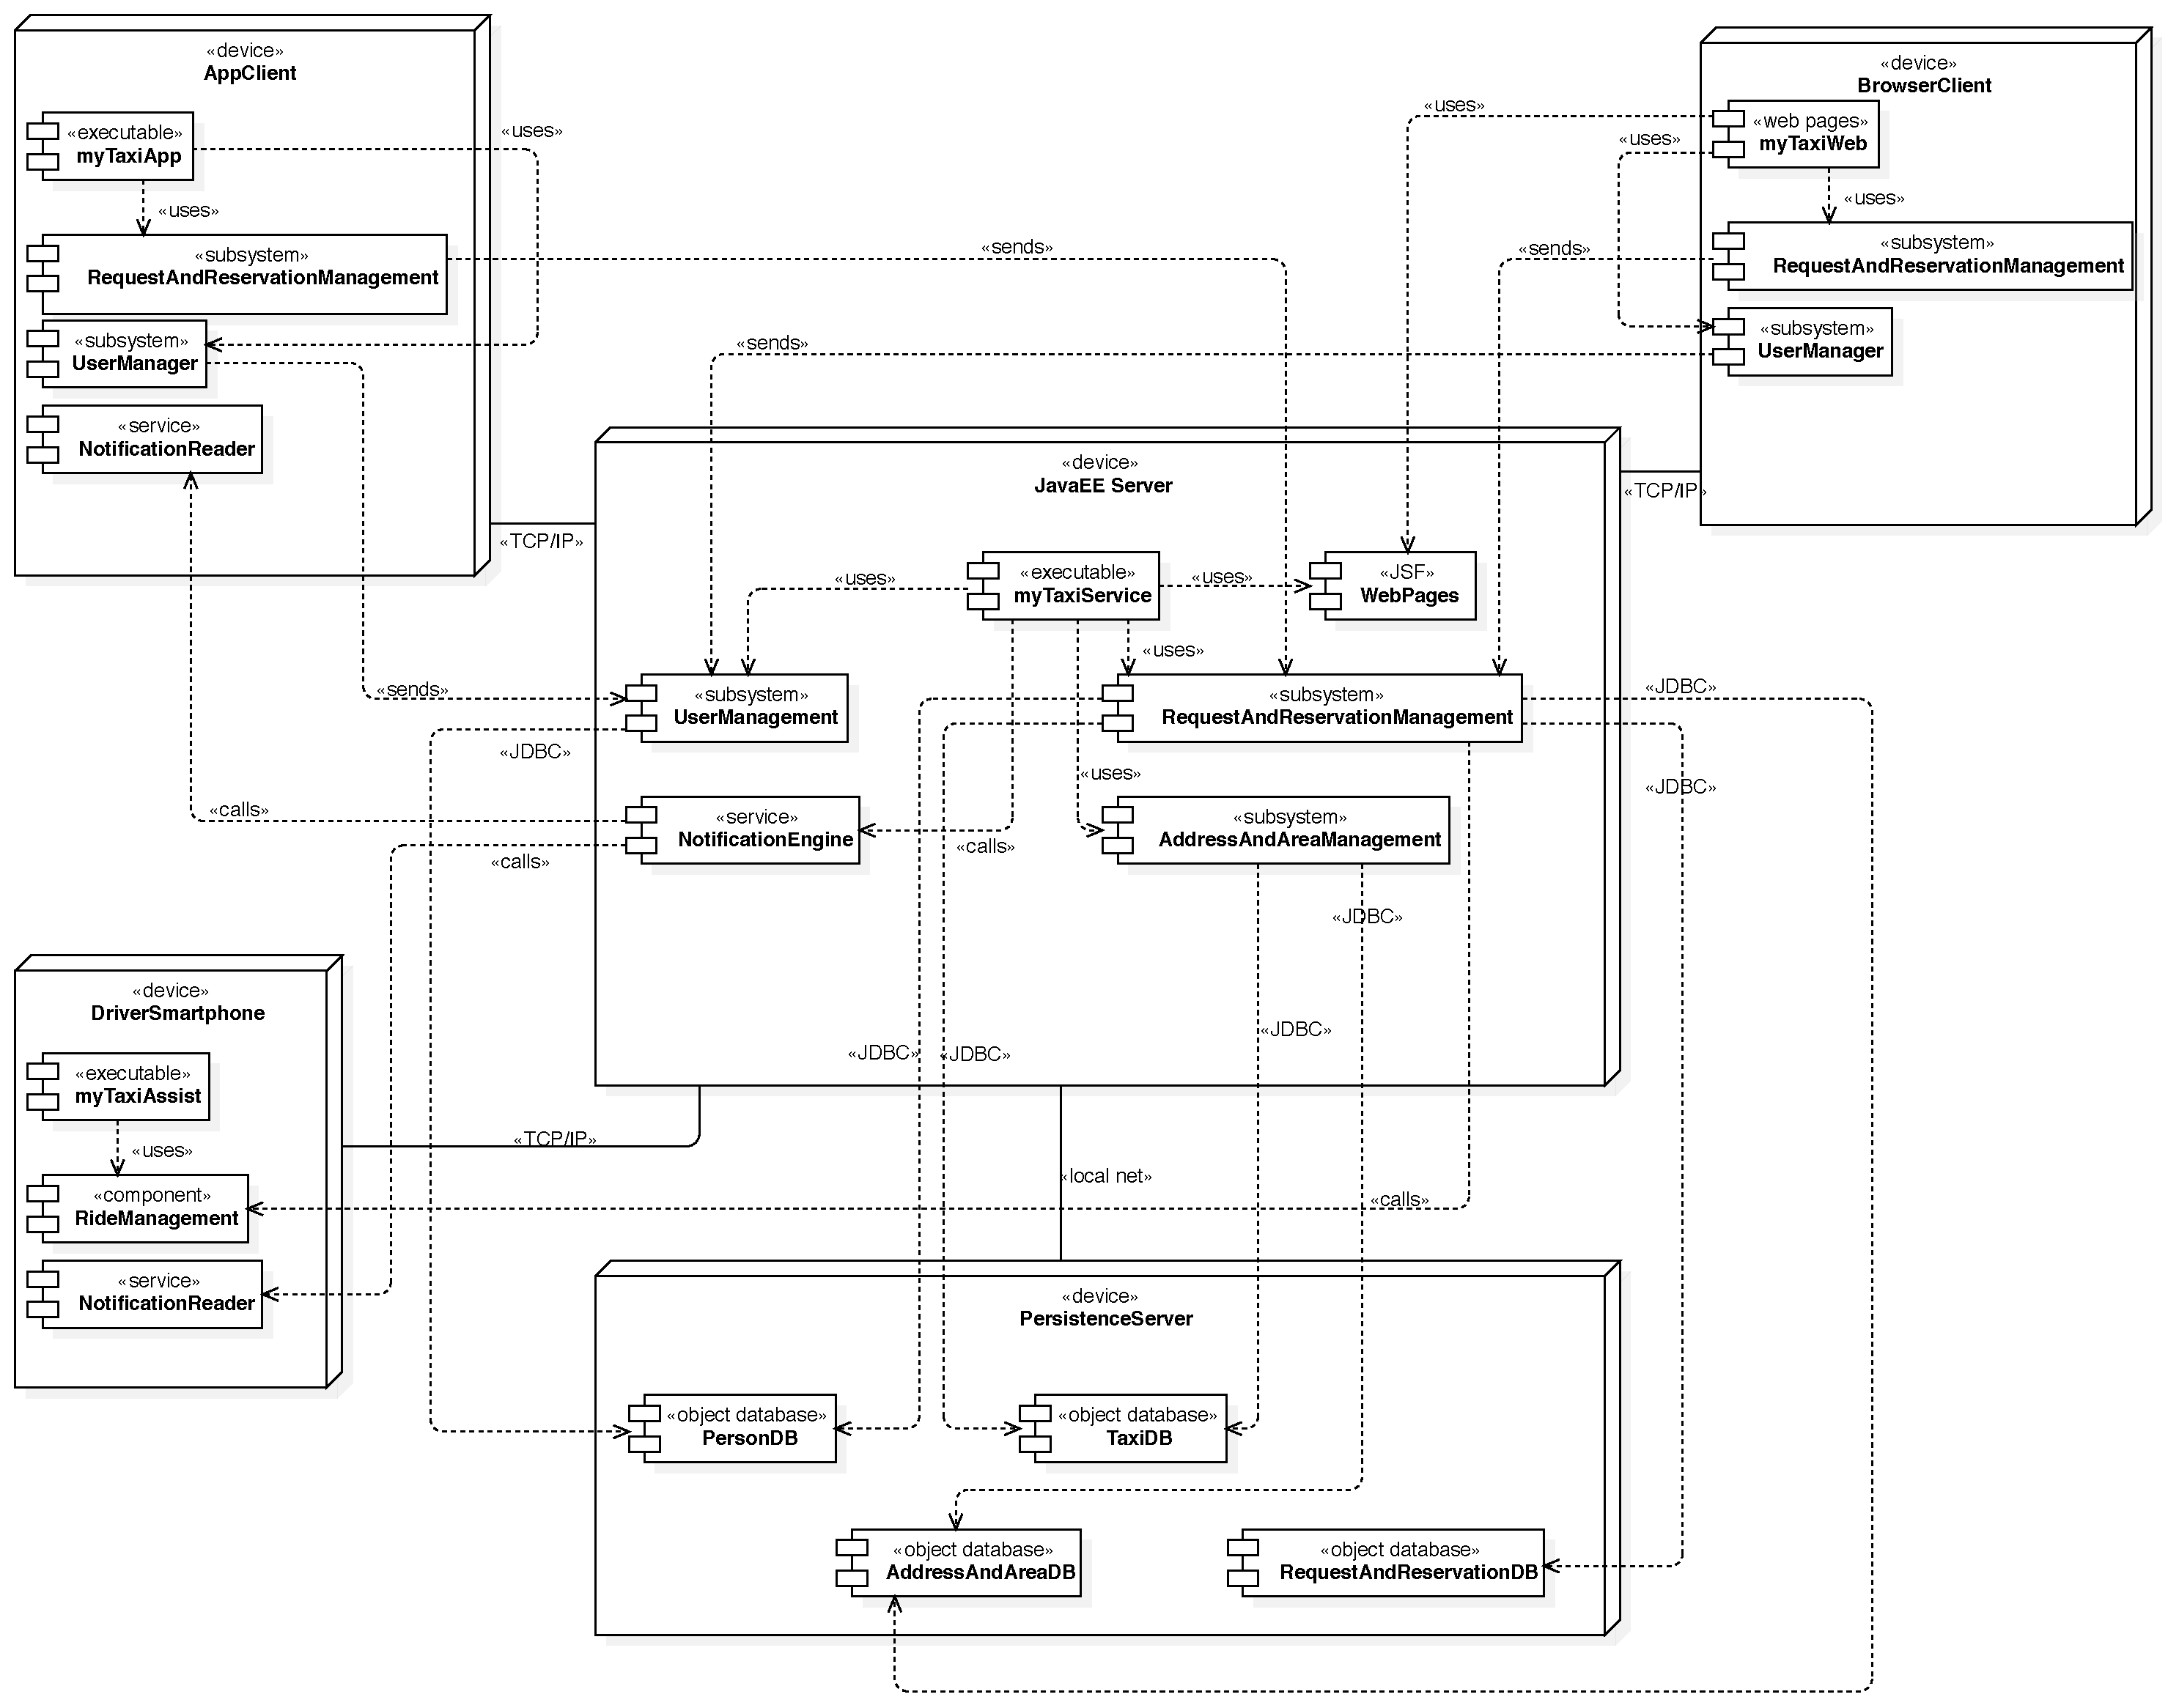
\includegraphics[width=\linewidth]{img/Deploy__DeploymentDiagram_4}%
	\caption{Deployment diagram.}\label{fig:deployment}%
\end{figure*}

To reflect the architecture shown in \cref{sec:highlevel}, the diagram develops over three types of hardware systems: \texttt{App\-Cli\-ent}, \texttt{Brows\-er\-Cli\-ent} and \texttt{Driver\-Smart\-phone} are the three possible client machines, then we have the \texttt{Java\-EE Ser\-ver}, intended for the business logic, and the \texttt{Per\-sist\-ence\-Ser\-ver}, which is a different machine, dedicated to the database.

The main interactions between the components have been drawn. Moreover, the nature of the various components (executable, service) has been specified, so as to give a comprehensive view on the architecture of the system.













\clearpage%TODO Remove.
\section{Runtime view}\label{sec:runtime}
%[You can use sequence diagrams to describe the way components interact to accomplish specific tasks typically related to your use cases.] [this is what you have in slide 9 plus sequence diagrams describing the way components behave in order to accomplish a certain activity]

Qui si è voluta presentare una visione delle istanze che possono essere attive sul sistema quando sono state effettuate due richieste, una tramite prenotazione (app) ed una diretta (web) alle quali per comodità è stato allocato lo stesso taxi (ipotizzate consecutive).

Alcune delle relazioni tra le istanze sono date per scontate per motivi di leggibilità (ad esempio il customer della reservation1 (customer1) è lo stesso della request1, ma non viene esplicitato alla request1).


\begin{figure*}%
	\centering%
	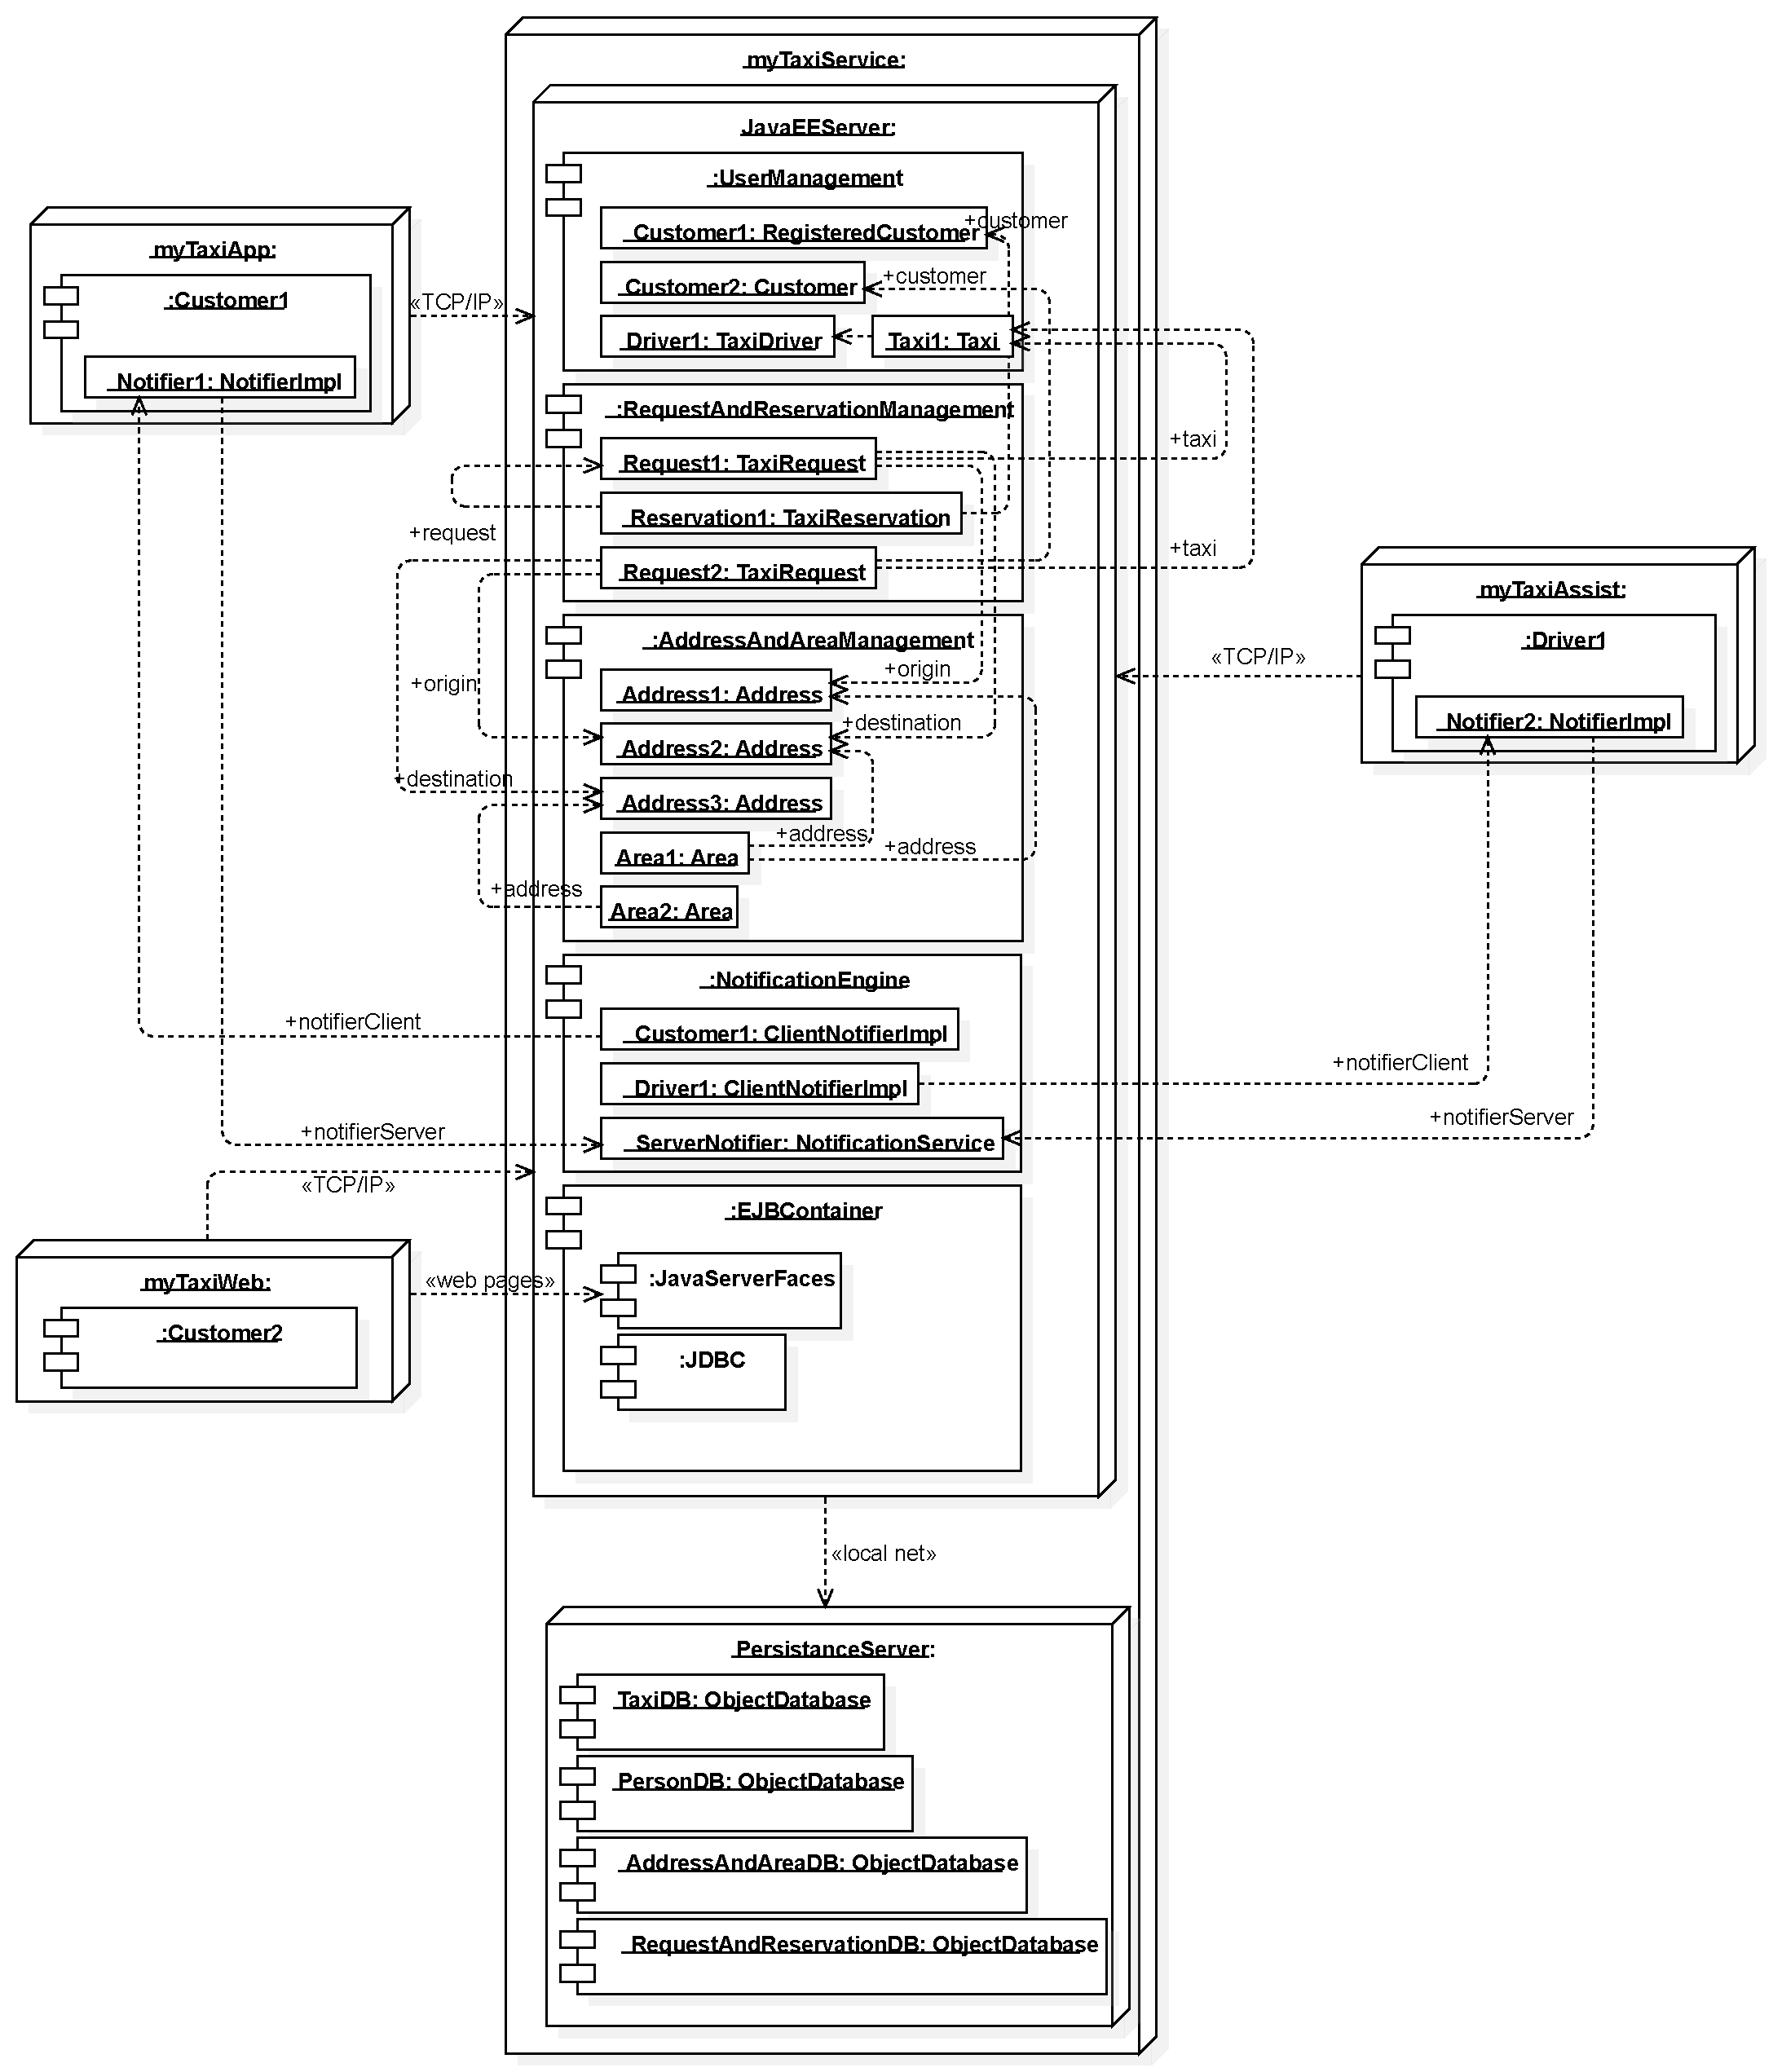
\includegraphics[width=\linewidth]{img/Runtime__RuntimeView_5}%
	\caption{Runtime view.}\label{fig:runtime}%
\end{figure*}



SEQUENCE

Questi diagrammi vogliono evidenziare il comportamento del sistema in due casi tipici (una richiesta ed una prenotazione), evidenziando gli scambi di messaggi e i metodi invocati tra i vari component del sistema.



\begin{figure*}%
	\centering%
	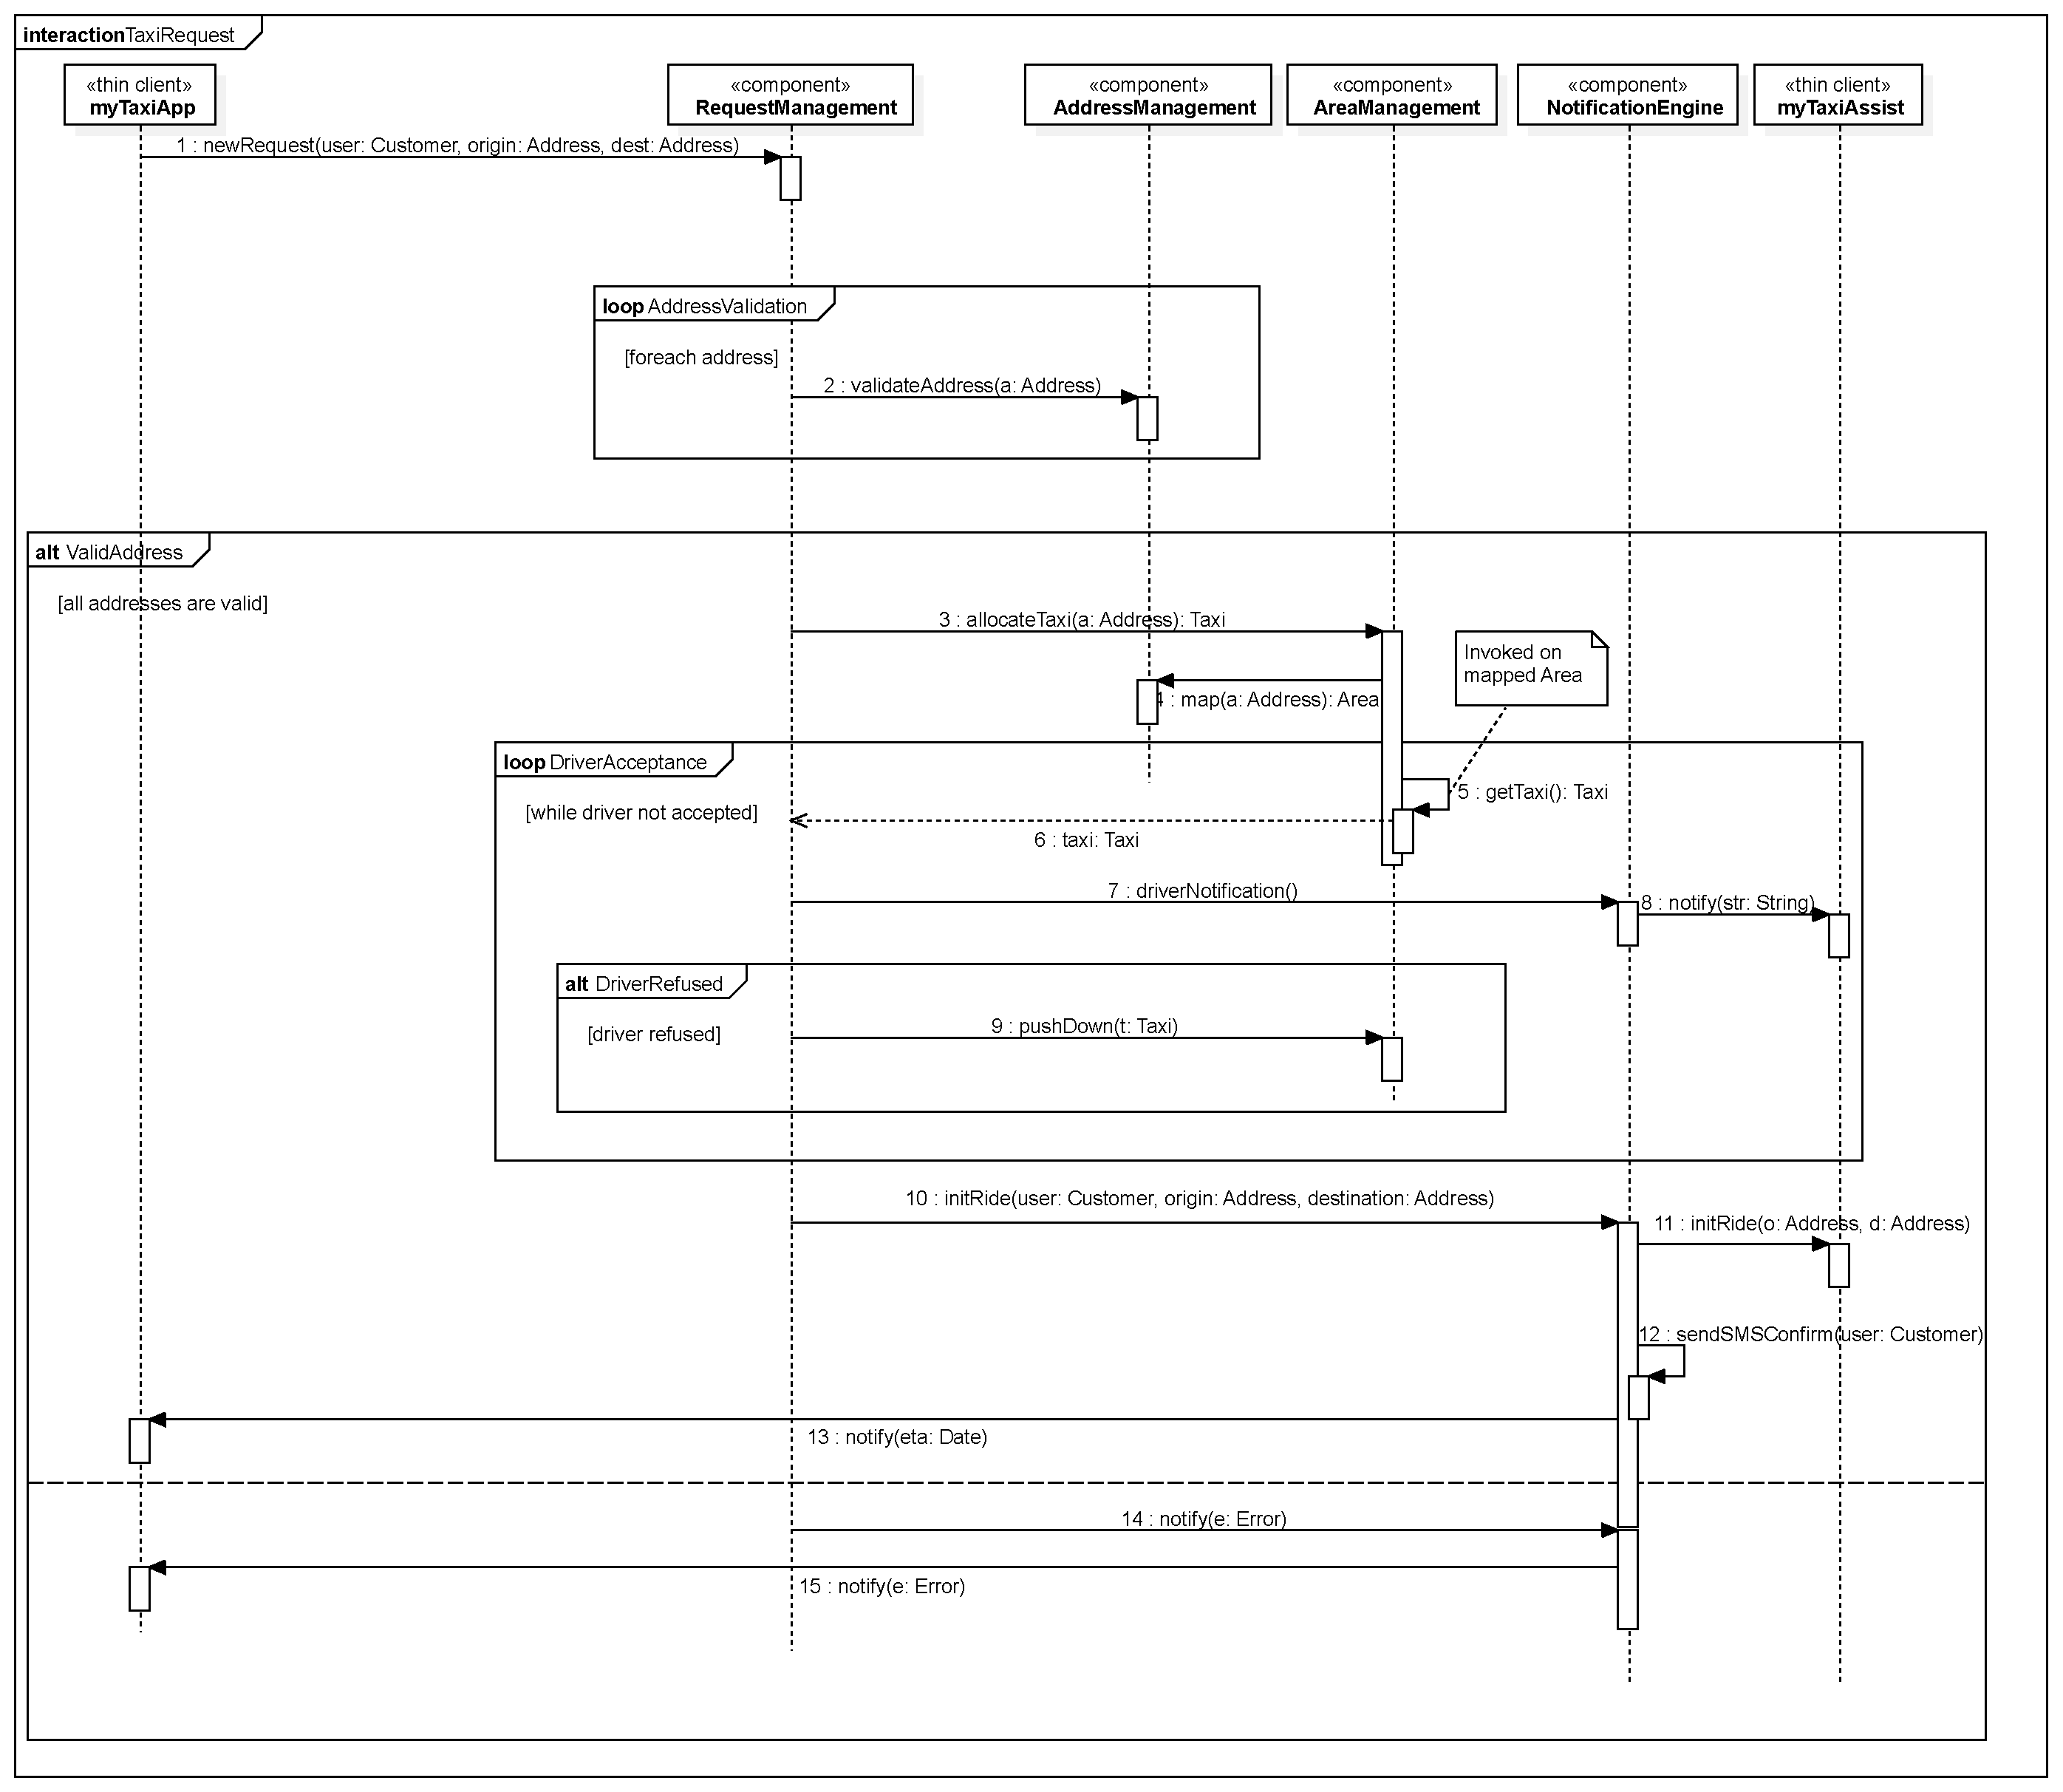
\includegraphics[width=\linewidth]{img/Sequence__Collaboration1__Interaction1__TaxiRequest_2}%
	\caption{Taxi request sequence diagram.}\label{fig:reqSequence}%
\end{figure*}

\begin{figure*}%
	\centering%
	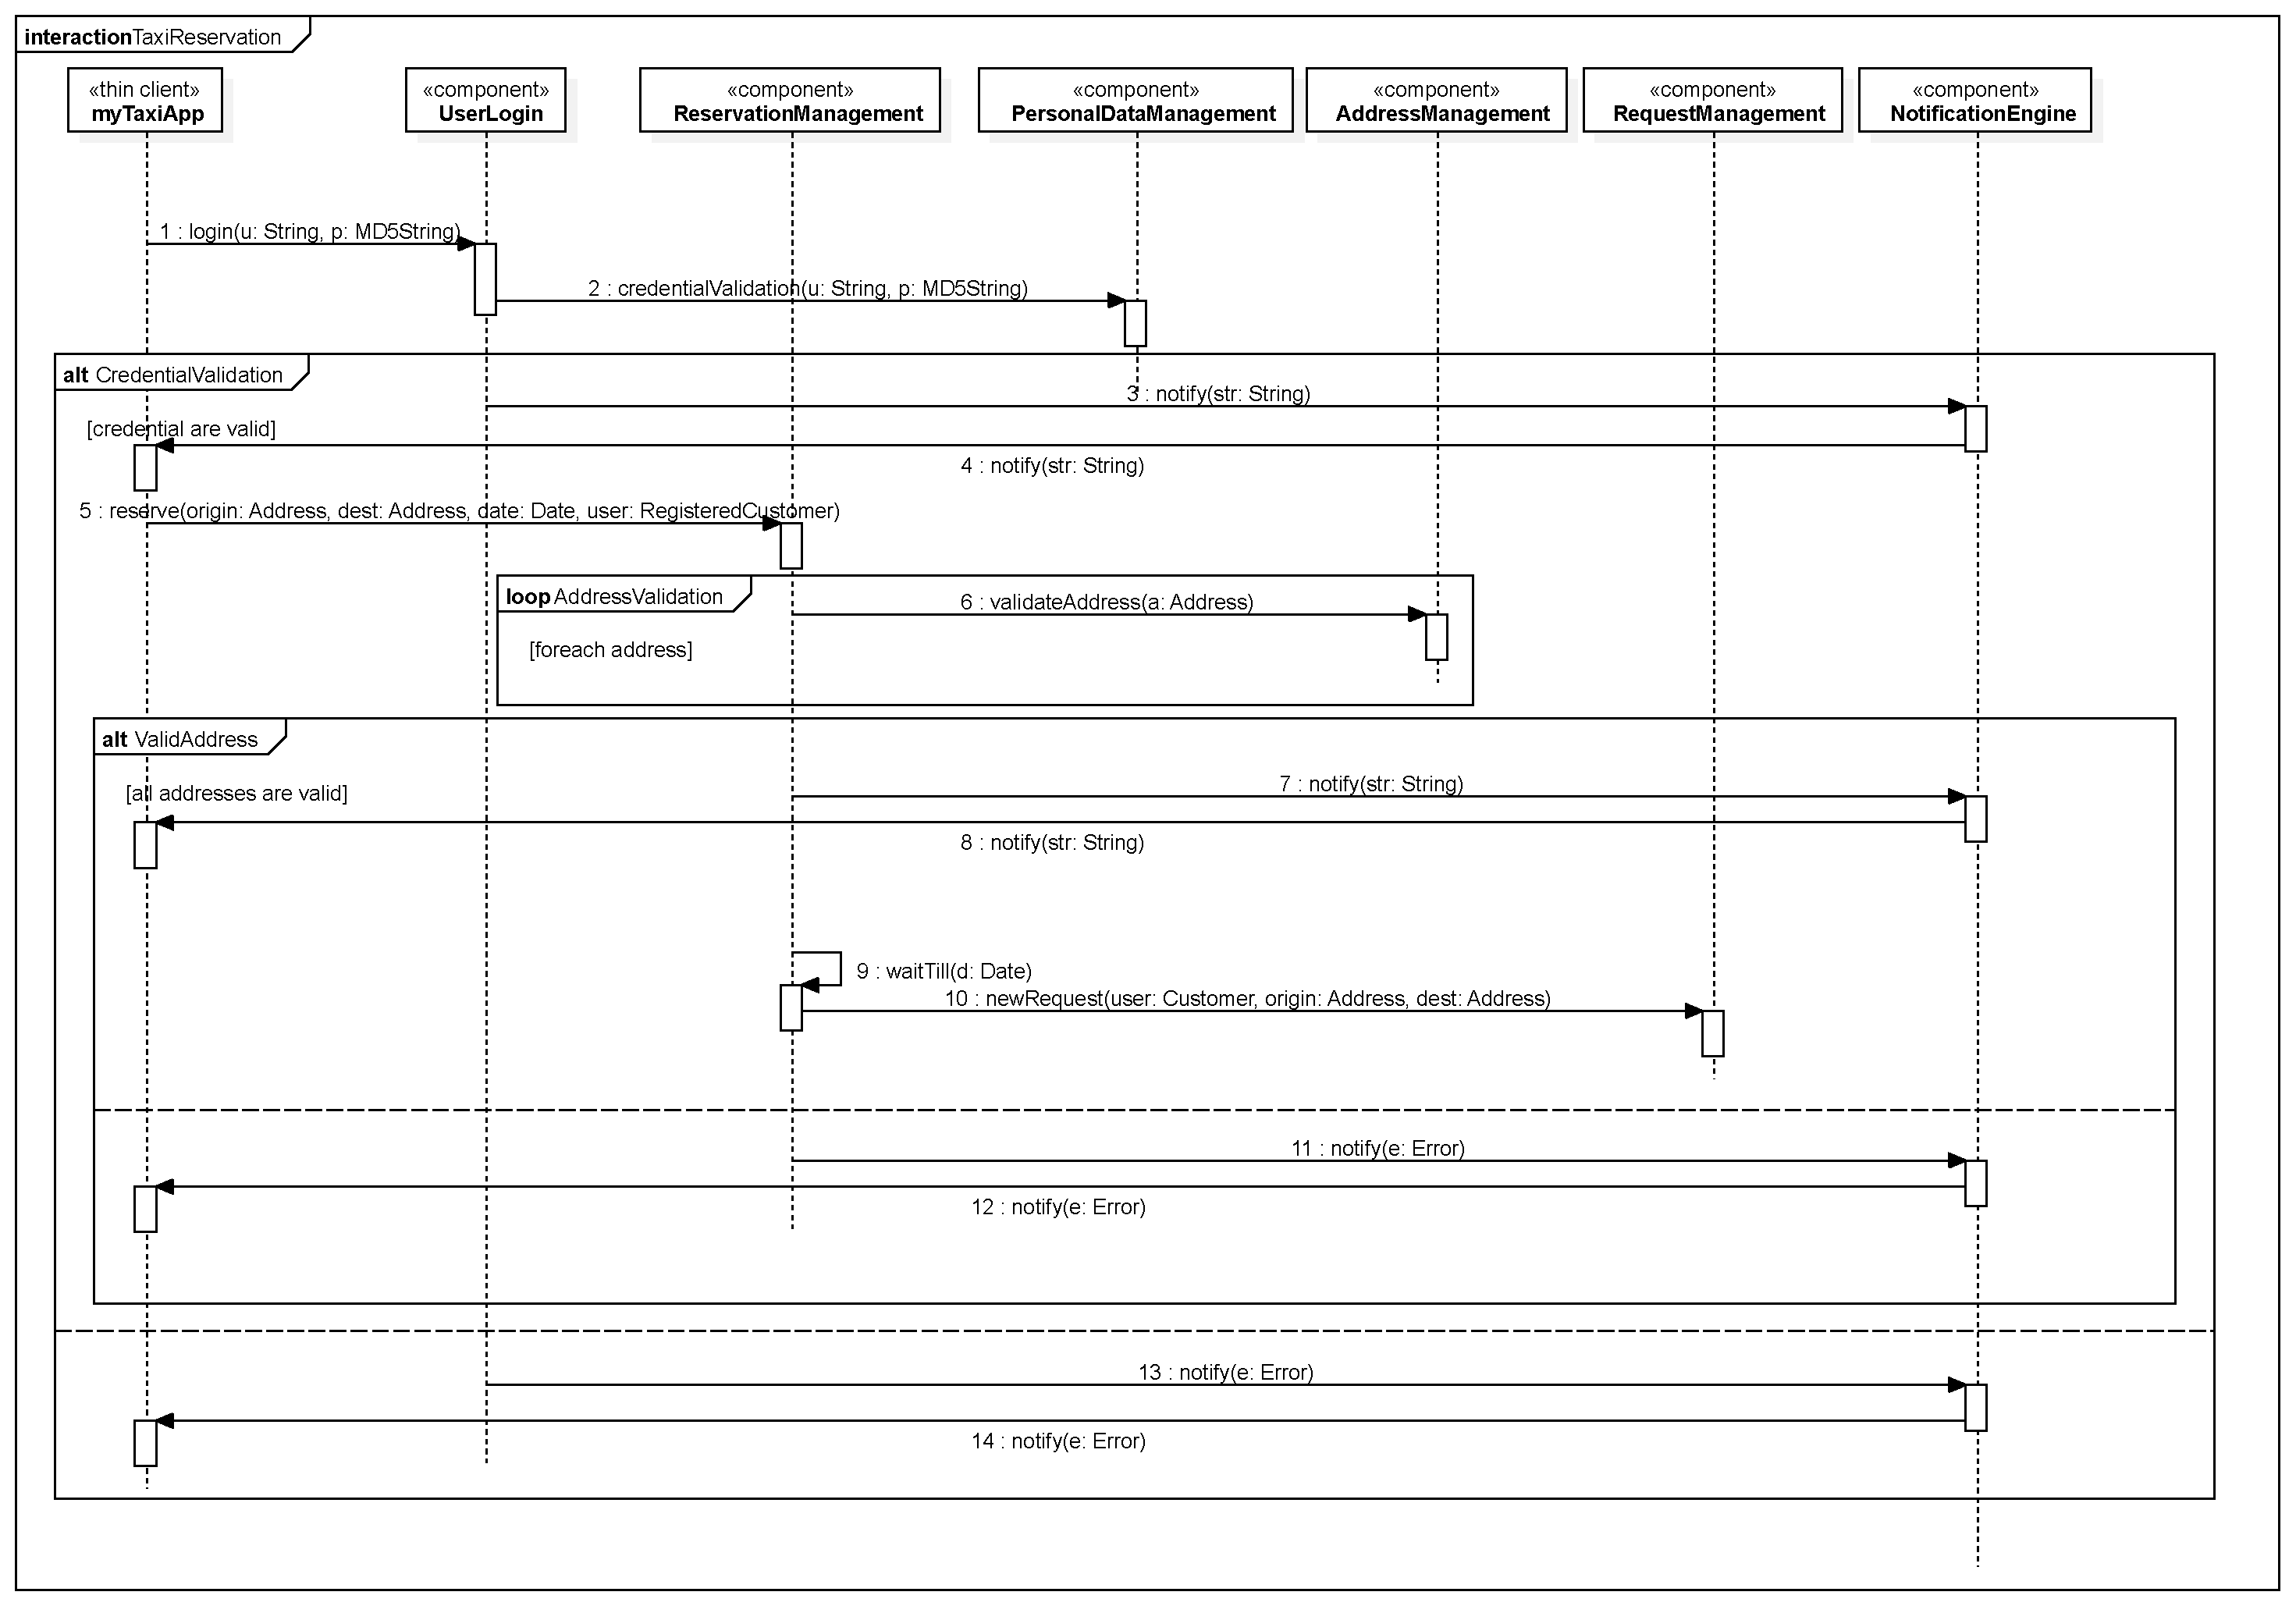
\includegraphics[width=\textwidth]{img/Sequence__Collaboration2__Interaction1__TaxiReservation_3}%
	\caption{Taxi reservation sequence diagram.}\label{fig:resSequence}%
\end{figure*}
























\clearpage%TODO Remove.
\section{Selected architectural styles and patterns}\label{sec:styles}
[Please explain which styles/patterns you used, why, and how.] [3-tier architecture STYLE; ]















\clearpage%TODO Remove.
\section{Other design decisions}\label{sec:decisions}
\lipsum[8]
